\begin{figure}[htbp]
  \centering
  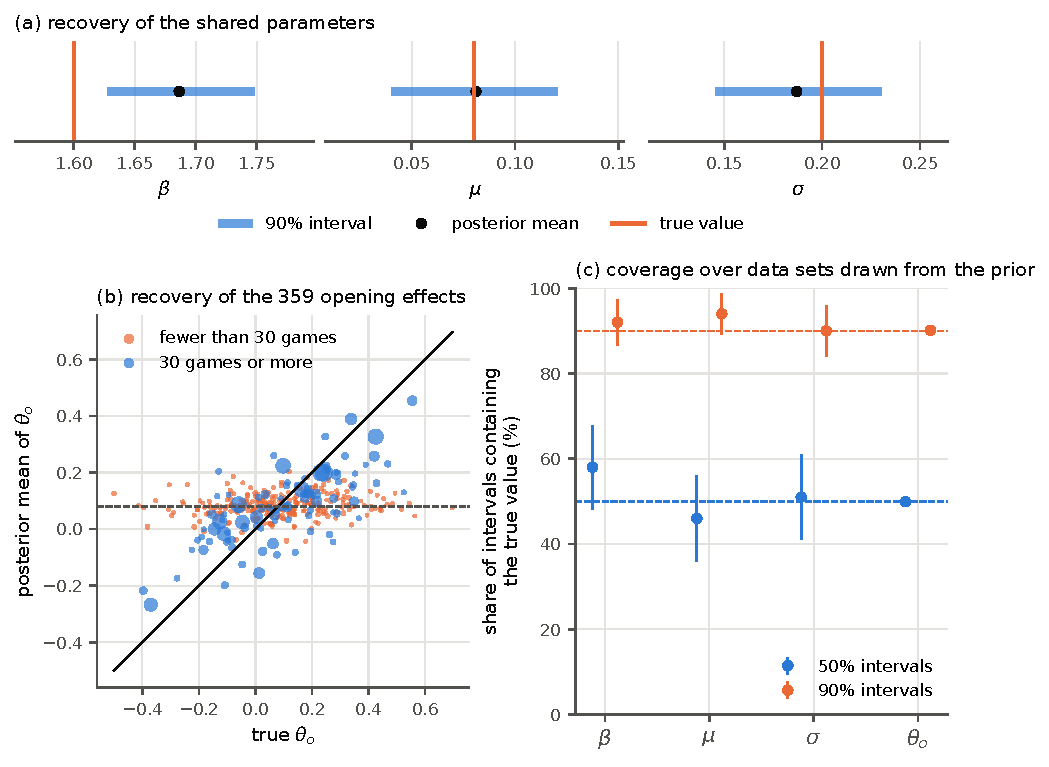
\includegraphics[width=\linewidth]{validation.pdf}
  \caption{Validation on simulated games, with the real rating gaps and openings and the results drawn from the model. (a): one data set simulated with chosen values (orange lines); the posterior mean (black) and the central 90\% interval (blue) of $\beta$, $\mu$ and $\sigma$. The 90\% interval of $\beta$ misses the true value 1.6 (posterior mean 1.686); over 40 repeated data sets with the same values, the 90\% interval of $\beta$ contains it 90\% of the time and the posterior mean is off by 0.008 on average (standard error 0.006), so the miss is chance and not a bias. (b): true opening effects of the same data set against their posterior means, with the area of each point proportional to the number of games and the identity line in black. Openings with few games are shrunk towards the true $\mu$ (dashed line), and openings with many games lie near the identity line; 88.9\% of the 90\% intervals contain the true value. (c): share of the 50\% and 90\% posterior intervals that contain the true value, over 100 data sets whose parameters are drawn from the prior, with $\pm 2$ standard errors; for $\theta_o$ the share is over all openings of all data sets. The shares match the nominal levels (dashed lines), as they should when the sampler is correct.}
  \label{fig:validation}
\end{figure}
